\documentclass[letterpaper,11pt]{article}
\oddsidemargin -1.0cm \textwidth 17.5cm

\usepackage[utf8]{inputenc}
\usepackage[activeacute,spanish, es-lcroman]{babel}
\decimalpoint
\usepackage{amsfonts,setspace}
\usepackage{amsmath}
\usepackage{amssymb, amsmath, amsthm}
\usepackage{comment}
\usepackage{float}
\usepackage{amssymb}
\usepackage{dsfont}
\usepackage{anysize}
\usepackage{multicol}
\usepackage{enumerate}
\usepackage{graphicx}
\usepackage[left=1.5cm,top=2cm,right=1.5cm, bottom=1.7cm]{geometry}
\setlength\headheight{1.5em} 
\usepackage{fancyhdr}
\usepackage{multicol}
\usepackage{hyperref}
\usepackage{wrapfig}
\usepackage{subcaption}
\usepackage{siunitx}
\usepackage{cancel}
\usepackage{mdwlist}
\usepackage{svg}
\pagestyle{fancy}
\fancyhf{}
\renewcommand{\labelenumi}{\normalsize\bfseries P\arabic{enumi}.}
\renewcommand{\labelenumii}{\normalsize\bfseries (\alph{enumii})}
\renewcommand{\labelenumiii}{\normalsize\bfseries \roman{enumiii})}


\begin{document}

\fancyhead[L]{\itshape{Facultad de Ciencias F\'isicas y Matem\'aticas}}
\fancyhead[R]{\itshape{Universidad de Chile}}

\begin{minipage}{11.5cm}
    \begin{flushleft}
        \hspace*{-0.6cm}\textbf{FI1000-1 Introducción a la Física Clásica}\\
        \hspace*{-0.6cm}\textbf{Profesora:} Paulina Lira\\
        \hspace*{-0.6cm}\textbf{Auxiliares:} Alejandro Cartes \& Juan Cristóbal Castro\\
        \hspace*{-0.6cm}\textbf{Ayudantes:} Francisca Bórquez \& Catalina Molina\\
    \end{flushleft}
\end{minipage}

\begin{picture}(2,3)
    \put(366, 10){
\includegraphics[scale=0.9]{2020-1/Imágenes/logo/dfi-fcfm.pdf}}
\end{picture}

\begin{center}
	\LARGE\textbf{Auxiliar \#12}\\
	\Large{Estática del Sólido {\tiny{b}}Rígido}
\end{center}

\vspace{-1cm}
\begin{enumerate}\setlength{\itemsep}{0.4cm}

\rfoot[]{pág. \thepage}

\item[]

\item Una tortuga de masa $m$ camina con velocidad constante $v_0$ sobre una barra de largo $L$ y masa $M$. La barra cuelga de sus extremos por cuerdas verticales sin masa. En $t=0$ la tortuga está en el extremo izquierdo de la barra.

\begin{multicols}{2}
    
    \begin{enumerate}
        \item Determine las tensiones de las cuerdas en función del tiempo
        
        \item Suponga que la cuerda de la izquierda es de acero, pero la de la derecha es un hilo común. Por eso, la cuerda de la derecha tiene una tensión de corte de $T_{max}$, ¿cuál es la distancia máxima que puede recorrer la tortuga sin que se caiga?
    \end{enumerate}
    
    \columnbreak
    
    \begin{figure}[H]
        \centering
        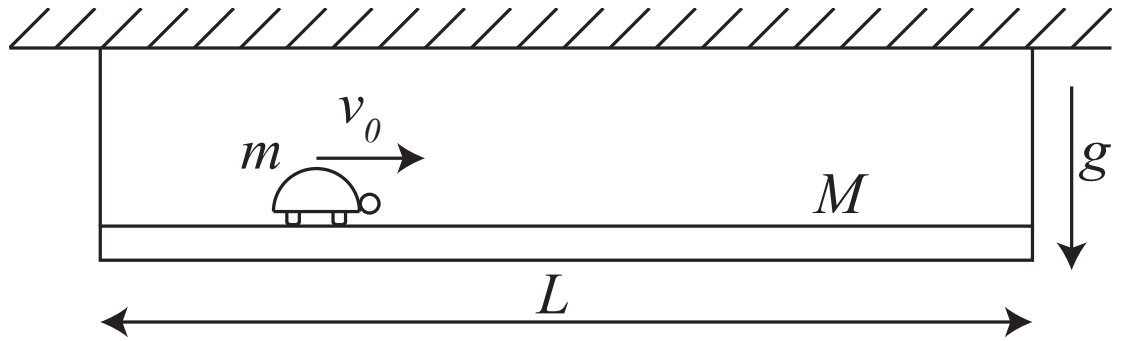
\includegraphics[width=0.9\linewidth]{2021-2/img/aux12/aux12-tortuga.PNG}
    \end{figure}
\end{multicols}

\item 
\begin{multicols}{2} Una barra de masa $M$ y largo $L$ se dobla en un ángulo $\alpha$ a una distancia $\lambda L$, con $\lambda \leq 1/2$, de uno de los extremos y se cuelga como se indica en la figura adjunta. La estructura se encuentra en equilibrio gracias a una masa $m$ que se cuelga en uno de los extremos.
    \begin{enumerate}
        \item Encuentre la tensión $T$ y el valor de $m$
        
        \item ¿Cómo cambian sus resultados si la barra, en vez de estar doblada en un ángulo $\alpha$ hacia abajo, está doblada hacia arriba?
    \end{enumerate}
    
    \columnbreak
    
    \begin{figure}[H]
        \centering
        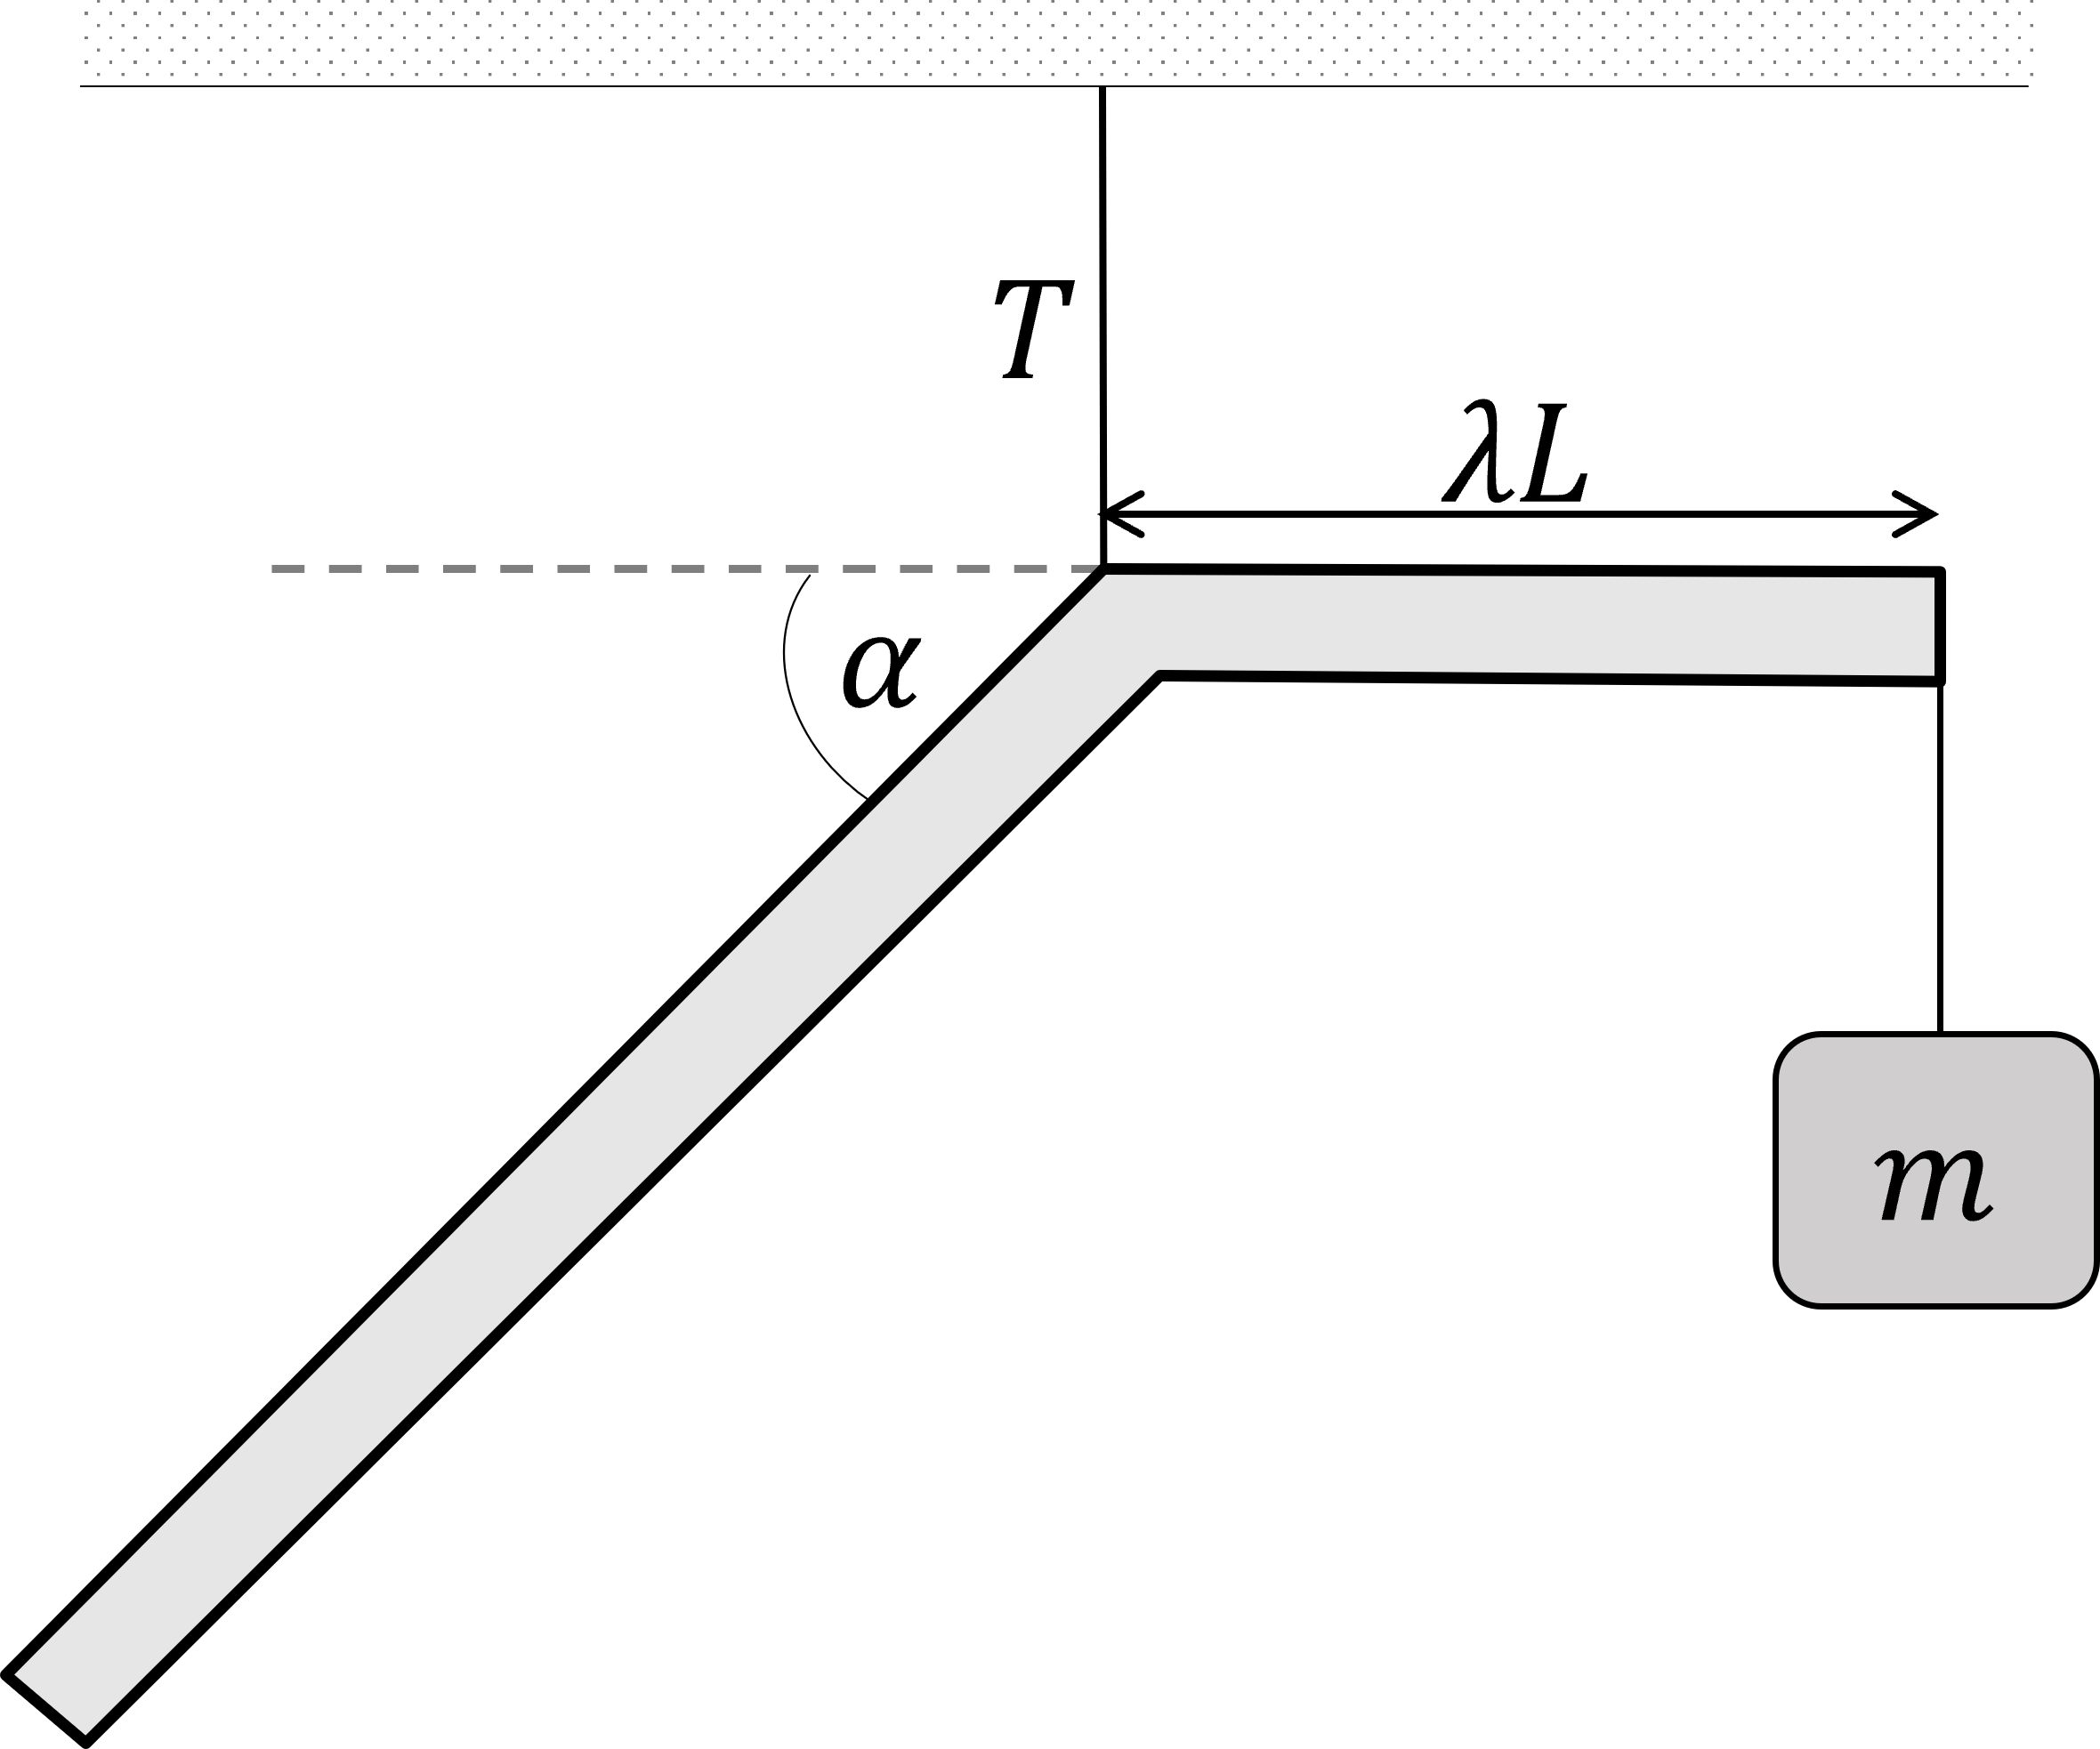
\includegraphics[width=0.6\linewidth]{2022-1/img/aux12/barra_dobla.png}
    \end{figure}
\end{multicols}

\item Considere una semiesfera de radio $R$ de masa $M$ que se encuentra sobre una superficie horizontal y apoyada contra una pared tal como se muestra en la figura adjunta. El centro de masas de una semiesfera homogénea queda sobre el eje de simetría y a una distancia ${b} = 3 R / 8$ de la base. Suponga que, entre la semiesfera y el suelo el coeficiente de roce estático es $\mu = 3 / 16$, mientras que entre la pared y la semiesfera el roce es nulo.

\begin{multicols}{2}
    \begin{enumerate}
        \item Realice un diagrama de cuerpo libre para la semiesfera.
        \item Encuentre la magnitud y dirección del torque, respecto al punto de apoyo $P$, ejercido por la fuerza de gravedad cuando la semiesfera está ladeada en un ángulo $\beta$.
        \item Encuentre la fuerza de roce entre la semi-esfera y el suelo
        \item Encuentre el ángulo de inclinación mínimo $\beta_{min}$ posible para que la semiesfera no resbale.
    \end{enumerate}
    
    \columnbreak
    
    \begin{figure}[H]
        \centering
        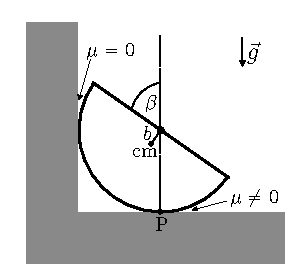
\includegraphics[width=0.6\linewidth]{2020-1/Imágenes/aux Extra-C2/semiesfera-torque.pdf}
    \end{figure}
\end{multicols}



% Para imágenes vectoriales -> el texto tiene que estar en LaTeX
% \begin{figure}[htbp]
%   \centering
%   \svgpath{../Imagenes/ejercicios}  -> .. irse pa'trás 
%   \includesvg{ej5.svg}
% \end{figure}

\end{enumerate}
\end{document}
